\documentclass[12pt]{notes}

% Command for Questions
%\question{}

% Command for Notes
% \note{}

% Code to create a minipage where you can type in class notes. 
%%\begin{minipage}[l][2cm][c]{\textwidth}
%\begin{comment}

%\end{comment}
%%\end{minipage}

\usepackage{listings}

% In order for the minted code to run, we had to create a new compilation routine called pdflatex+shellEscape.
% This includes a --shell-escape command which should ONLY be used when pygmentized is required as it compromises security. 
% We also had to add pygmentize (a python package) to the system path (BEFORE miktex) and then restart the computer. 
\usepackage{minted}
\usemintedstyle{borland}
\lstset{language=SAS, 
  breaklines=true,  
  basicstyle=\ttfamily\bfseries,
  columns=fixed,
  keepspaces=true,
  identifierstyle=\color{blue}\ttfamily,
  keywordstyle=\color{cyan}\ttfamily,
  stringstyle=\color{purple}\ttfamily,
  commentstyle=\color{green}\ttfamily,
  } 

% \begin{minted}{sas}
% \end{minted}

% Begin Document
%==============================================================================
\begin{document}
% Include the Title of the Handout
\ntitle{2.1: Introduction to Simple Linear Regression}

See \textbf{Handout 2.1.1} for information regarding the Toluca power company example.

% Include Numbered Sections
\section{Why Linear Regression?}

\nspace
Linear regression is good for: 
\begin{itemize}
\item \textbf{Inference:} determine if there is a statistically significant linear relationship between two variables, while possibly accounting for the effect of additional variables. 
\begin{itemize}
\item Example: after accounting for the effects of square footage and age, are lot size and home sale price significantly linearly related?  
\end{itemize} 
\item \textbf{Prediction:} use variables that are ``easy'' to measure to predict variables that are harder to measure.  
\begin{itemize}
\item Example: Use elevation (easy to measure) to predict annual snow accumulation (hard to measure). 
\end{itemize} 
\end{itemize}

\nspace
Linear regression only works for variables that share a statistical relationship.

\nspace
Terminology: 

\begin{itemize}
\item Y - response variable
\item $X_i$ - predictor variables
\item $\epsilon$ - error (or difference) term
\item $\beta_i$ - model parameters (true values are unknown and are estimated)
\end{itemize}

\nspace
Linear Regression focuses on finding appropriate estimates of the model parameters ($b_i$):

\nspace
The idea is that we want to select paramater estimates that make the predicted values of $Y$ ($\hat{Y}$) close to the actual values of $Y$.

\section{Ordinary Least Squares (OLS) Regression}
\textit{If assumptions regarding residuals are satisfied} (more in Handout 2.2), then the OLS estimates of the model parameters are ``best.''

\nspace
What does it mean to be ``best''?
\begin{itemize}
\item \textbf{unbiased} - given an infinite number of different samples of data, the average of my estimates will be equal to true (and unknown) value of the parameter. 
\begin{itemize}
\item In other words, my estimates are ``centered'' on the truth. 
\end{itemize}
\item \textbf{minimum variance} - the variation in the estimate from sample to sample is the smallest of all possible estimation methods. 
\end{itemize}

\subsection*{Applications - Toluca Example:} 
Let $X$ represent the lot size and let $Y$ represent the total work hours. Based on the initial scatterplot, we assume that the relationship between $X$ and $Y$ can be modeled as 

\[Y = \beta_0 + \beta_1X + \epsilon\]

\nspace
OLS seeks to minimize:
\[
Q = \sum_{i=1}^n\left(Y_i - \hat{Y}_i \right)^2,
\]

which requires us to select estimates $b_0$ and $b_1$ that minimize
\[
Q = \sum_{i=1}^n\left(Y_i - \left(b_0 + b_1X_i \right) \right)^2 = f(\mathbf{X}).
\]

We can use multivariable calculus to find the minimum of Q by finding the critical points, i.e. 
\[\nabla Q = \nabla f(\mathbf{X}) = 0.\]

The single critical point that minimizes $Q$ is 
\begin{align*}
b_1 &= \frac{\sum_i (X_i - \bar{X})(Y_i - \bar{Y})}{\sum_i\left(X_i - \bar{X}\right)^2} \\
b_0 &= \bar{Y} - b_1\bar{X}.
\end{align*} 

Obtain OLS estimates automatically in SAS with:

\begin{minted}{sas}
proc reg data=toluca;
  model workhours = lotsize;
  title1 'Simple linear model';
run;
\end{minted}

\nspace
Equation Estimates:

\begin{minipage}[l][1cm][c]{\textwidth}
%\begin{comment}
\note{$b_0 = 62.37$, $b_1 = 3.57$}
%\end{comment}
\end{minipage}

\nspace
Model Equation:

\begin{minipage}[l][1cm][c]{\textwidth}
%\begin{comment}
\note{$\hat{Y} = 62.37 + 3.57(lotSize)$}
%\end{comment}
\end{minipage}

\subsection*{The Critical Assumption}
OLS least squares hinges on the assumption that

\[\epsilon \stackrel{iid}{\sim} N(0, \sigma^2)\]

\begin{itemize}
\item \textbf{independent:} Knowing the value of one of the model residuals tells you nothing about any of the others. 
\item \textbf{identically distributed:} All of the residuals come from the same distribution.
\item \textbf{Normal Distribution:} The model residuals follow a normal (bell shaped) distribution. 
\item \textbf{zero mean:} The average of the residuals is zero (unbiased estimates). 
\item \textbf{constant variance:} The spread of the residuals about the line is the same across the range of $X$ and the range of predicted values. 
\end{itemize}

\textit{If the assumptions hold,} then the simple linear regression can be visualized as in Figure \ref{wicklin}.

\begin{figure}[H]
\centering
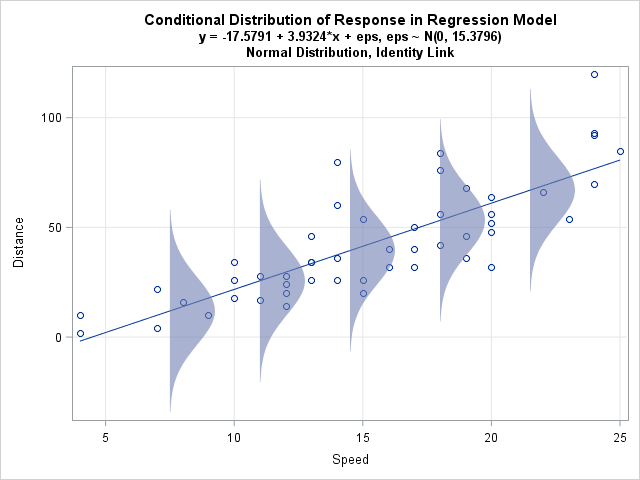
\includegraphics[width = 0.6\textwidth]{figures/module2/normalPic_wicklin.png}
\caption{Sample visualization taken from Rick Wicklin on The DO Loop.}
\label{wicklin}
\end{figure}

In other words, $Y$ follows a normal distribution with a center that is conditional on $X$. 

\subsection*{Estimating $\sigma$}
Estimating the variance about the regression line:
\begin{itemize}
\item Allows us to get a measure of the model fit: lower relative MSE $\rightarrow$ better model. 
\item All significance tests of model coefficients are based on our estimate of $\sigma$. 
\end{itemize} 

\subsubsection*{Estimation of $\epsilon$ in Theory}
Suppose that $\epsilon_1, \epsilon_2, \ldots, \epsilon_n$ were an observed sample from some population. (In practice, $\epsilon$ is estimated as the residuals of our OLS model, represented as $e_i$.)

\nspace
We could then estimate $\Var(\epsilon)$ as 
\[\frac{1}{n-1}\sum_{i=1}^n\left(\epsilon_i - \bar{\epsilon}\right)^2\].

\nspace
Note that the variance calculation requires the estimation of $\mu_\epsilon = \bar{\epsilon} = \frac{1}{n}\sum_i\epsilon_i.$

\nspace
This calculation ``constrains'' one of the $\epsilon_i$. This means that if we know $\bar{epsilon}$ and $\epsilon_1, \ldots \epsilon_{n-1},$ then we can know $\epsilon_n$. 

\nspace
We call the number of unconstrained observations the ``degrees of freedom'' (DF). 

\nspace
Every time you estimate a parameter, \textbf{you lose one degree of freedom.}

 % Code to create a minipage where you can type in class notes. 
\begin{minipage}[l][2cm][c]{\textwidth}
%\begin{comment}
\note{Think of observations as currency. We spend money to estimate things and our degrees of freedom are the leftover cash.}
%\end{comment}
\end{minipage}

\subsubsection*{Estimation of $\epsilon$ in Practice}

Why is it that we can't directly obtain the values of $\epsilon$?

\begin{minipage}[l][2cm][c]{\textwidth}
%\begin{comment}
\note{We don't know the true regression line, so we cannot know the true values of epsilon.}
%\end{comment}
\end{minipage}

We can obtain estimates of the residuals $e_i$ through the regression line: 
\[
e_i = Y_i - \hat{Y}_i = Y_i - (b_0 + b_1X_i).
\]

\nspace
OLS, by design, makes $\sum_ie_i = 0 \rightarrow \bar{e} = 0$, meaning I don't have to spend any DF to obtain $\bar{e}$. 


% End the Document
%==============================================================================
\end{document}

\nspace
\question{(Review) What is the difference between a functional and a statistical relationship?}

\begin{minipage}[l][3cm][c]{\textwidth}
%\begin{comment}
\note{Functional: $Y = f(X)$ (no scatter).}

\nspace
\note{Statistical: $Y = f(X) + \epsilon$ (scatter about the line)}
%\end{comment}
\end{minipage}

\nspace
\question{(Review) What does it mean to be linear?}

\nspace
\note{\[Y = \beta_0 + \sum_i\beta_if(X_i)\]}

\question{(Individual) If I start with $n$ degrees of freedom, how many DF do I have left after calculating the residuals in the Toluca example?}

\begin{minipage}[l][2cm][c]{\textwidth}
%\begin{comment}
\note{$n-2$ since I spent 1 to calculate $b_0$ and another to calculate $b_1$.}
%\end{comment}
\end{minipage}

\question{(Individual) Now suppose that my model equation was actually $\hat{Y} = b_0 + b_1X_1 + b_2X_2$ how many DF would have left after calculating the residuals?}

\begin{minipage}[l][2cm][c]{\textwidth}
%\begin{comment}
\note{$n-3$ since I spent 1 to calculate $b_0$, another to calculate $b_1$, and a third to calculate $b_2$.}
%\end{comment}
\end{minipage}

We estimate $\sigma^2$ in the Toluca example as: 
\[\hat{\sigma}^2 = s^2 = \frac{1}{df_E}\sum_{i=1}^ne_i^2 = \frac{1}{n-2}\sum_{i=1}^n\left(e_i-\bar{e}\right)^2\]

We call this estimate the \textbf{``mean square error''} or MSE. 

\begin{minipage}[l][2cm][c]{\textwidth}
%\begin{comment}
\note{Toluca Example: $\hat{\sigma}^2 = 2383.72$}
%\end{comment}
\end{minipage}

